% ============================================================
% Final Project Presentation
% Project 08: Exploratory Scientific Literature Search
% Course: CSC15012 - Applications of NLP in Industry
% Student: Le Dinh Minh Quan - 23127460 - 23CNTThuc
% ============================================================

\documentclass[10pt,aspectratio=169]{beamer}

\mode<presentation>
{
  \usetheme{Madrid}
  \usecolortheme{seahorse}
  \usefonttheme{default}
  \setbeamertemplate{navigation symbols}{}
  \setbeamertemplate{caption}[numbered]
  \setbeamertemplate{footline}[frame number]
}

% ---- Packages ----
\usepackage[english]{babel}
\usepackage[utf8]{inputenc}
\usepackage{amsmath}
\usepackage{graphicx}
\usepackage{booktabs}
\usepackage{xcolor}
\usepackage{hyperref}
\usepackage{xurl}
\usepackage{tikz}
\usepackage{pgfplots}
\pgfplotsset{compat=1.18}
\usetikzlibrary{shapes.geometric, arrows.meta, positioning, fit, backgrounds, shadows}
\usepackage{listings}
\lstset{
  basicstyle=\ttfamily\scriptsize,
  breaklines=true,
  frame=single,
  backgroundcolor=\color{gray!10},
  keywordstyle=\color{blue},
  commentstyle=\color{green!60!black},
  stringstyle=\color{red!70!black},
  showstringspaces=false,
  tabsize=2
}

% ---- HCMUS LOGO ----
% Upload logo_hcmus.png to Overleaf to display the logo (top-right of every slide).
% If the file is missing, no logo is shown (no error).
\IfFileExists{logo_hcmus.png}{\logo{\includegraphics[height=0.7cm]{logo_hcmus.png}}}{}

% ---- TITLE METADATA ----
\title[Project 08: Scientific Literature Search]{Project 08: Exploratory Scientific Literature Search}
\subtitle{A Fine-tuned Dense Retriever + Hybrid Search Engine + Exploratory-Search Agent}
\author[Le Dinh Minh Quan]{Le Dinh Minh Quan \\ \small ID: 23127460 -- Class: 23CNTThuc}
\institute[HCMUS]{Vietnam National University Ho Chi Minh City \\ University of Science -- Faculty of Information Technology \\ \small Course: CSC15012 -- Applications of NLP in Industry}
\date{2026}

\begin{document}

% ============================================================
% SLIDE 1: TITLE
% ============================================================
\begin{frame}
  \titlepage
\end{frame}

% ============================================================
% SLIDE 2: OUTLINE
% ============================================================
\begin{frame}{Outline}
\begin{columns}[T]
\begin{column}{0.5\textwidth}
\begin{enumerate}
  \item Business Problem \& Motivation
  \item Proposed NLP Solution \& Success Metrics
  \item System Architecture
  \item Repository \& Tech Stack
  \item Data Management
  \item Training \& Autopilot Workflow
  \item Evaluation: Metrics \& Baselines
  \item Offline-vs-Colab Results
\end{enumerate}
\end{column}
\begin{column}{0.5\textwidth}
\begin{enumerate}
  \setcounter{enumi}{8}
  \item Agentic AI Component (D1--D4)
  \item Agent Example Interaction
  \item Deployment
  \item Ethics, Privacy \& Fairness
  \item Monitoring \& Continual Learning
  \item Key Takeaways \& Future Work
  \item Resources \& Thank You
\end{enumerate}
\end{column}
\end{columns}
\end{frame}

% ============================================================
% SLIDE 3: BUSINESS PROBLEM & MOTIVATION
% ============================================================
\begin{frame}{1. Business Problem \& Motivation}
\begin{block}{Context}
Scientific output grows faster than anyone can read. Today's tools fail in two ways: \textbf{keyword search misses the concept}, and \textbf{a flat ranked list offers no exploration}.
\end{block}

\begin{columns}[T]
\begin{column}{0.5\textwidth}
\textbf{Pain points}
\begin{itemize}
  \item BM25 is blind to paraphrase / concept
  \item No sense of the \emph{shape} of results
  \item No sub-topics, neighbours, broaden/narrow
  \item User often doesn't know the right query yet
\end{itemize}
\end{column}
\begin{column}{0.5\textwidth}
\textbf{Users \& jobs-to-be-done}
\begin{itemize}
  \item Researchers -- find concept matches
  \item Analysts -- map a field
  \item Lit-review authors -- coverage (Recall)
  \item Citation expansion -- fan out from a paper
\end{itemize}
\end{column}
\end{columns}
\end{frame}

% ============================================================
% SLIDE 4: PROPOSED NLP SOLUTION + SUCCESS METRICS
% ============================================================
\begin{frame}{2. Proposed NLP Solution \& Success Metrics}
\begin{block}{Solution}
Exploratory search: a query returns a ranked list \textbf{plus} facets, topic clusters, related rails and broaden/narrow guidance -- backed by a \textbf{fine-tuned dense bi-encoder}, a \textbf{hybrid (dense+BM25) engine}, and a \textbf{4-decision agent}.
\end{block}

\begin{table}[h]
\centering\small
\begin{tabular}{lll}
\toprule
\textbf{Type} & \textbf{Metric} & \textbf{Target} \\
\midrule
Business & Time-to-first-relevant & Down vs.\ keyword search \\
Business & Exploration depth & $\geq 1$ facet/cluster/related per session \\
Business & Zero-result rate & $<2\%$ (D2 coverage gate) \\
Technical & \textbf{nDCG@10} (headline) & Beat BM25 \emph{and} zero-shot base \\
Technical & Recall@\{1,5,10\}, MRR@10 & Reported (coverage, not precision-only) \\
Technical & Latency & Hot path tens of ms; end-to-end sub-second \\
\bottomrule
\end{tabular}
\end{table}

\footnotesize \textbf{Core claim}: fine-tuning the retriever beats both BM25 and the zero-shot encoder on nDCG@10 -- largest margin on \emph{conceptual} queries.
\end{frame}

% ============================================================
% SLIDE 5: SYSTEM ARCHITECTURE (TikZ)
% ============================================================
\begin{frame}{3. System Architecture}
\centering
\resizebox{0.96\linewidth}{!}{%
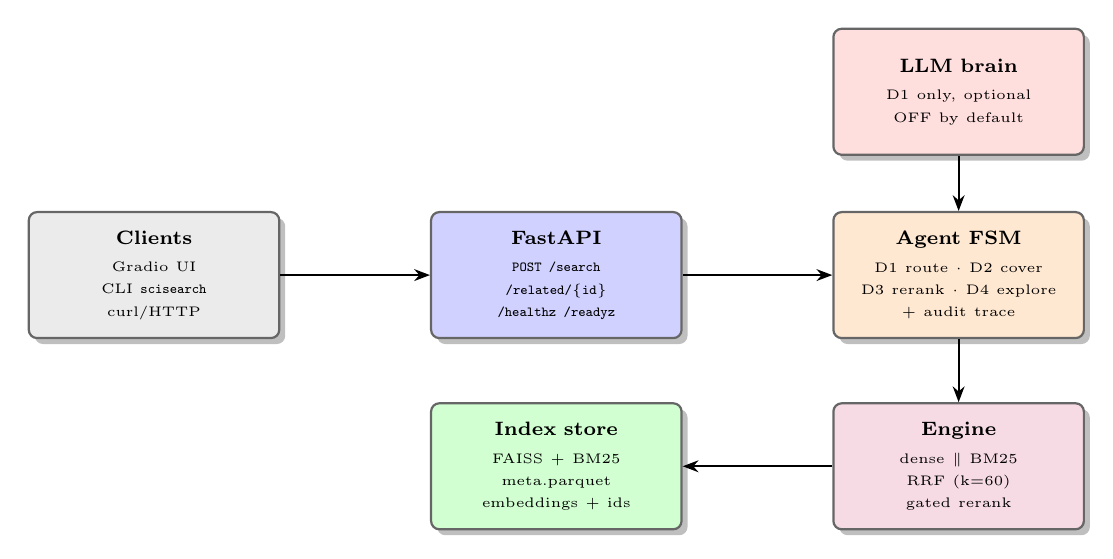
\begin{tikzpicture}[
  node distance=0.8cm and 1.9cm,
  box/.style={rectangle, draw=black!60, rounded corners=3pt, thick,
              text width=2.9cm, minimum height=1.6cm, align=center,
              inner sep=4pt, font=\scriptsize, drop shadow},
  clientbox/.style={box, fill=gray!16},
  apibox/.style={box, fill=blue!18},
  agentbox/.style={box, fill=orange!18},
  enginebox/.style={box, fill=purple!14},
  databox/.style={box, fill=green!18},
  brainbox/.style={box, fill=red!13},
  arrow/.style={-{Stealth[length=2mm]}, thick}
]
\node[clientbox] (cli) {\textbf{Clients}\\[2pt]{\tiny Gradio UI}\\{\tiny CLI \texttt{scisearch}}\\{\tiny curl/HTTP}};
\node[apibox, right=of cli] (api) {\textbf{FastAPI}\\[2pt]{\tiny \texttt{POST /search}}\\{\tiny \texttt{/related/\{id\}}}\\{\tiny \texttt{/healthz /readyz}}};
\node[agentbox, right=of api] (agent) {\textbf{Agent FSM}\\[2pt]{\tiny D1 route $\cdot$ D2 cover}\\{\tiny D3 rerank $\cdot$ D4 explore}\\{\tiny + audit trace}};
\node[enginebox, below=of agent] (engine) {\textbf{Engine}\\[2pt]{\tiny dense $\parallel$ BM25}\\{\tiny RRF (k=60)}\\{\tiny gated rerank}};
\node[databox, below=of api] (store) {\textbf{Index store}\\[2pt]{\tiny FAISS + BM25}\\{\tiny meta.parquet}\\{\tiny embeddings + ids}};
\node[brainbox, above=0.7cm of agent] (brain) {\textbf{LLM brain}\\[2pt]{\tiny D1 only, optional}\\{\tiny OFF by default}};

\draw[arrow] (cli.east) -- (api.west);
\draw[arrow] (api.east) -- (agent.west);
\draw[arrow] (agent.south) -- (engine.north);
\draw[arrow] (engine.west) -- (store.east);
\draw[arrow] (brain.south) -- (agent.north);
\end{tikzpicture}%
}

\vspace{0.2cm}
\scriptsize \textbf{One brain, three faces}: API, UI, and CLI all delegate to the \emph{same} agent + engine. The optional Anthropic brain advises only D1 and is OFF by default $\Rightarrow$ zero external calls in the default config.
\end{frame}

% ============================================================
% SLIDE 6: REPOSITORY & TECH STACK
% ============================================================
\begin{frame}[fragile]{4. Repository Structure \& Tech Stack}
\begin{columns}[T]
\begin{column}{0.55\textwidth}
\textbf{GitHub repo} (public, MIT) \\
\scriptsize \url{https://github.com/ledinhminhquan/08_Scientific_Literature_Search}

\vspace{0.15cm}
\begin{lstlisting}[basicstyle=\ttfamily\tiny]
src/scisearch/
|-- config.py  cli.py  logging_utils.py
|-- data/      samples(offline) corpus pairs download
|-- models/    bm25 retriever vector_store reranker
|              model_registry
|-- search/    hybrid(RRF) facets expand engine
|-- training/  train_retriever evaluate tune metrics
|-- agent/     state policy(D1-D4) tools
|              llm_orchestrator search_agent
|-- api/       schemas dependencies main ui app_combined
|-- analysis/ autoreport/ monitoring/ automation/ grading/
configs/ data/ models/ tests/ docs/ notebooks/ app/ deploy/
Dockerfile docker-compose.yml pyproject.toml README.md
\end{lstlisting}
\end{column}
\begin{column}{0.45\textwidth}
\textbf{Tech stack}
\begin{itemize}\scriptsize
  \item Python 3.11, Git + GitHub
  \item \texttt{sentence-transformers} (MNRL)
  \item \textbf{\texttt{BAAI/bge-small-en-v1.5}} (MIT, 33.4M, 384-dim)
  \item fallback \texttt{all-MiniLM-L6-v2}
  \item \texttt{cross-encoder/ms-marco-MiniLM-L-6-v2} (rerank)
  \item FAISS (\texttt{faiss-cpu}) + \texttt{rank-bm25}
  \item scikit-learn (KMeans/TF-IDF)
  \item FastAPI + Uvicorn, Gradio
  \item Docker + compose, HF Space
  \item Anthropic brain (optional, OFF)
  \item Colab H100 (auto-profiles A100/L4/T4)
\end{itemize}
\end{column}
\end{columns}
\end{frame}

% ============================================================
% SLIDE 7: DATA MANAGEMENT
% ============================================================
\begin{frame}{5. Data Management}
\begin{columns}[T]
\begin{column}{0.52\textwidth}
\textbf{Datasets} (ids verified on HF Hub)
\begin{itemize}\scriptsize
  \item Corpus: \texttt{gfissore/arxiv-abstracts-2021} -- \textbf{CC0-1.0}, 2.0M rows (title+abstract+categories+authors+versions)
  \item Real eval: \texttt{BeIR/scifact} -- \textbf{CC-BY-SA} \textcolor{red!70!black}{[!]} (eval only; attribution + share-alike)
  \item Offline fallback: built-in $\sim$40 NLP papers (MIT)
\end{itemize}

\textbf{Synthetic spine / pairs}
\begin{itemize}\scriptsize
  \item No labels $\Rightarrow$ self-supervised pairs
  \item Lexical: \texttt{title $\rightarrow$ abstract}
  \item Conceptual: \texttt{first-sentence $\rightarrow$ paper}
  \item Negatives: in-batch (MNRL); \texttt{no\_duplicates}
\end{itemize}
\end{column}
\begin{column}{0.48\textwidth}
\textbf{Preprocessing \& splits}
\begin{itemize}\scriptsize
  \item Indexed text = title + abstract
  \item Category list $\rightarrow$ readable field facets
  \item Dedup (also anti-overfitting)
  \item Leakage-free query/corpus split
\end{itemize}

\textbf{Offline self-check (verified)}
\begin{itemize}\scriptsize
  \item Runs with no GPU, no network
  \item TF-IDF retriever + identity reranker + numpy store
  \item All 4 decisions fire; ``dense passage retrieval'' $\rightarrow$ DPR paper \#1
\end{itemize}

\scriptsize \textbf{Limits}: arXiv-only, English, 2021 cutoff, title/abstract only.
\end{column}
\end{columns}
\end{frame}

% ============================================================
% SLIDE 8: TRAINING & AUTOPILOT WORKFLOW
% ============================================================
\begin{frame}{6. Training \& Autopilot Workflow (Colab/H100)}
\centering
\begin{tikzpicture}[
  node distance=0.16cm,
  step/.style={rectangle, draw=black!60, rounded corners=2pt, thick,
              minimum width=11.6cm, minimum height=0.52cm, align=center, font=\scriptsize},
  setup/.style={step, fill=gray!15},
  train/.style={step, fill=orange!15},
  eval/.style={step, fill=blue!15},
  deploy/.style={step, fill=green!15},
  arrow/.style={-{Stealth[length=1.8mm]}, thick}
]
\node[setup] (s1) {\textbf{1. Setup}: mount Drive, install deps, \textbf{auto-profile GPU} (H100 bs256 / A100 bs128 / L4 bs64 / T4 bs32)};
\node[setup, below=of s1] (s2) {\textbf{2. Data}: load \texttt{arxiv-abstracts-2021}, facet metadata, generate (title$\rightarrow$abstract, first-sent$\rightarrow$paper) pairs};
\node[train, below=of s2] (s3) {\textbf{3. Fine-tune}: \texttt{SentenceTransformerTrainer} + MNRL, in-batch negatives, bf16+tf32, resume-safe};
\node[eval, below=of s3] (s4) {\textbf{4. Evaluate}: BM25 + zero-shot + fine-tuned on \texttt{BeIR/scifact} (Recall@\{1,5,10\}, MRR@10, nDCG@10)};
\node[eval, below=of s4] (s5) {\textbf{5. Hybrid + rerank}: FAISS index, RRF fuse (k=60), gated cross-encoder rerank};
\node[eval, below=of s5] (s6) {\textbf{6. Agent + analysis}: FSM D1--D4 with audit trace; latency benchmark; per-query error analysis};
\node[deploy, below=of s6] (s7) {\textbf{7. Auto-gen} \texttt{report.pdf} + \texttt{slides.pptx} + metric tables};
\node[deploy, below=of s7] (s8) {\textbf{8. Self-grade \& bundle} (\texttt{scisearch grade})};
\foreach \a/\b in {s1/s2,s2/s3,s3/s4,s4/s5,s5/s6,s6/s7,s7/s8}
  \draw[arrow] (\a) -- (\b);
\end{tikzpicture}

\vspace{0.12cm}
\scriptsize \textbf{One-button} on Colab H100. \texttt{bge-small} fine-tunes in $\approx$minutes--$\sim$1\,h. Resume-safe; \texttt{load\_best\_model\_at\_end} on the IR metric (not loss).
\end{frame}

% ============================================================
% SLIDE 9: EVALUATION -- METRICS & BASELINES
% ============================================================
\begin{frame}{7. Evaluation: Metrics \& Baselines}
\begin{columns}[T]
\begin{column}{0.5\textwidth}
\textbf{Three rankers compared}
\begin{itemize}\small
  \item \textbf{BM25} -- lexical Okapi (exact terms)
  \item \textbf{Zero-shot base} -- un-fine-tuned bge/MiniLM
  \item \textbf{Fine-tuned} -- the system we ship
\end{itemize}
BM25 vs.\ dense isolates \emph{lexical-vs-semantic}; zero-shot vs.\ fine-tuned isolates \emph{fine-tuning}.

\vspace{0.15cm}
\textbf{Metrics}
\begin{itemize}\small
  \item \textbf{nDCG@10} -- headline (graded, rank-aware)
  \item Recall@\{1,5,10\} -- coverage
  \item MRR@10 -- rank of first relevant
\end{itemize}
\end{column}
\begin{column}{0.5\textwidth}
\textbf{RRF fusion} (rank-based, scale-invariant)
\[
\text{score}(d)=\sum_{r}\frac{1}{k+\text{rank}_r(d)},\; k=60
\]
\footnotesize Intent biases fusion by \emph{duplicating} the preferred ranking (keyword $\rightarrow$ BM25, conceptual $\rightarrow$ dense).

\vspace{0.15cm}
\textbf{Per-query error buckets}
\begin{itemize}\scriptsize
  \item \textbf{Dense wins} $\rightarrow$ justifies fine-tuning
  \item \textbf{BM25 wins} $\rightarrow$ justifies keeping BM25 in RRF
  \item \textbf{Both fail} $\rightarrow$ target for D2 coverage gate
\end{itemize}
\end{column}
\end{columns}
\end{frame}

% ============================================================
% SLIDE 10: OFFLINE-vs-COLAB RESULTS
% ============================================================
\begin{frame}{8. Results: Offline Smoke Test vs.\ Colab Verdict}
\begin{columns}[T]
\begin{column}{0.52\textwidth}
\textbf{Headline table} (filled by Colab/H100 on \texttt{BeIR/scifact})
\begin{table}[h]
\centering\scriptsize
\begin{tabular}{lccc}
\toprule
\textbf{Metric} & \textbf{BM25} & \textbf{Zero-shot} & \textbf{Fine-tuned} \\
\midrule
nDCG@10 & [Colab] & [Colab] & \textbf{[Colab]} \\
Recall@1 & [Colab] & [Colab] & [Colab] \\
Recall@5 & [Colab] & [Colab] & [Colab] \\
Recall@10 & [Colab] & [Colab] & [Colab] \\
MRR@10 & [Colab] & [Colab] & [Colab] \\
\bottomrule
\end{tabular}
\end{table}
\scriptsize Success $=$ fine-tuned $\geq$ both baselines on nDCG@10, largest margin on conceptual queries.
\end{column}
\begin{column}{0.48\textwidth}
\textbf{Offline smoke test (verified today)}
\begin{itemize}\scriptsize
  \item Built-in $\sim$40-paper corpus, no GPU/network
  \item Whole pipeline runs; all 4 decisions fire
  \item Metrics \textbf{saturate} (few candidates $\Rightarrow$ all rankers $\approx$ rank-1) -- \emph{expected}
\end{itemize}

\vspace{0.1cm}
\centering
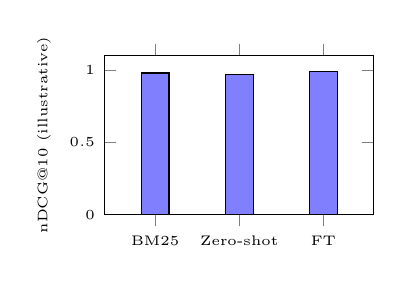
\begin{tikzpicture}
\begin{axis}[
  ybar, width=5.0cm, height=3.6cm,
  ymin=0, ymax=1.1,
  symbolic x coords={BM25, Zero-shot, FT},
  xtick=data, x tick label style={font=\tiny},
  ylabel={\tiny nDCG@10 (illustrative)},
  bar width=10pt, enlarge x limits=0.3,
  ytick={0,0.5,1.0}, y tick label style={font=\tiny}
]
\addplot[fill=blue!50] coordinates {(BM25,0.98) (Zero-shot,0.97) (FT,0.99)};
\end{axis}
\end{tikzpicture}

\scriptsize \emph{Mini-corpus saturates near 1.0; differentiation appears at scale (the Colab run).}
\end{column}
\end{columns}
\end{frame}

% ============================================================
% SLIDE 11: AGENTIC AI COMPONENT
% ============================================================
\begin{frame}{9. Agentic AI Component -- Deterministic FSM (D1--D4)}
\centering
\begin{tikzpicture}[
  node distance=0.16cm,
  step/.style={rectangle, draw=black!60, rounded corners=2pt, thick,
              text width=11.4cm, minimum height=0.5cm, align=center, font=\scriptsize, inner sep=3pt},
  dec/.style={step, fill=red!12},
  ret/.style={step, fill=blue!15},
  rer/.style={step, fill=purple!15},
  exp/.style={step, fill=green!15},
  arrow/.style={-{Stealth[length=1.8mm]}, thick}
]
\node[dec] (d1) {\textbf{D1 -- Query-type routing} (\textbf{tool} + optional brain): intent \{keyword/conceptual/hybrid\} + filters $\rightarrow$ biases RRF};
\node[ret, below=of d1] (s1) {\textbf{Retrieve + Fuse} (\textbf{tool}): dense $\parallel$ BM25 $\rightarrow$ \texttt{rrf\_fuse(k=60)}};
\node[dec, below=of s1] (d2) {\textbf{D2 -- Coverage gate} (\textbf{decision}): too few / low top-sim $\rightarrow$ expand (abbrev + PRF) + re-retrieve; backstops zero-result $<2\%$};
\node[dec, below=of d2] (d3) {\textbf{D3 -- Rerank gate} (\textbf{decision}): small head margin $\rightarrow$ rerank; else skip (saves +150--400 ms)};
\node[rer, below=of d3] (s2) {\textbf{Rerank} (\textbf{tool}, gated): cross-encoder ms-marco-MiniLM-L-6-v2 re-scores top-k};
\node[exp, below=of s2] (d4) {\textbf{D4 -- Exploration} (\textbf{multi-step reasoning}): facets + KMeans/TF-IDF clusters + related NN $\rightarrow$ broaden/narrow/related};
\foreach \a/\b in {d1/s1,s1/d2,d2/d3,d3/s2,s2/d4}
  \draw[arrow] (\a) -- (\b);
\end{tikzpicture}

\vspace{0.12cm}
\scriptsize \textbf{Rubric coverage}: multi-step reasoning (D1, D4), tool usage (understand/retrieve/rerank/explore), decision-making on intermediate outputs (D2, D3). Deterministic $\Rightarrow$ reproducible + gradeable; full audit trace in \texttt{decisions[]}.
\end{frame}

% ============================================================
% SLIDE 12: AGENT EXAMPLE INTERACTION
% ============================================================
\begin{frame}[fragile]{10. Agent Example Interaction (validated offline)}
\textbf{Query: \texttt{"dense passage retrieval"}}
\begin{lstlisting}[basicstyle=\ttfamily\tiny]
D1 understand : concept phrase, no field filter -> intent = CONCEPTUAL
                (fusion up-weights the dense ranking)
Retrieve+RRF  : dense (bge-small, fine-tuned) || BM25 -> rrf_fuse(k=60),
                dense ranking duplicated to honor the conceptual bias
D2 coverage   : plenty of results + strong head similarity -> coverage_ok
D3 rerank     : head close/ambiguous (small head_margin) -> RERANK
                cross-encoder ms-marco-MiniLM-L-6-v2 re-scores top-k
D4 explore    : KMeans/TF-IDF clusters + arXiv-field facets +
                dense-NN related rail -> suggestion = related

Outcome: Dense Passage Retrieval paper ranks #1; all four decisions fire
         and are recorded in decisions[]; response = results + facets +
         clusters + related rails + suggestion strip.
\end{lstlisting}

\scriptsize Ran on the built-in mini-corpus (TF-IDF retriever + identity reranker) -- correct intent routing, all D1--D4 fire, full audit trace.
\end{frame}

% ============================================================
% SLIDE 13: DEPLOYMENT
% ============================================================
\begin{frame}{11. Deployment}
\textbf{Five interchangeable surfaces -- one engine, one agent}
\begin{itemize}\small
  \item \textbf{FastAPI}: \texttt{POST /search}, \texttt{GET /related/\{id\}}, \texttt{/healthz /readyz /version}
  \item \textbf{Gradio UI}: search box + facet/cluster sidebar + decision log (mounted at \texttt{/ui})
  \item \textbf{CLI} (\texttt{scisearch}): data/pairs/train/evaluate/search/demo-agent/serve/autopilot/grade
  \item \textbf{Docker / Compose}: \texttt{python:3.11-slim}, \texttt{docker compose up --build}
  \item \textbf{HF Space} (app/): hosted-demo packaging; models pulled on first boot
\end{itemize}

\begin{columns}[T]
\begin{column}{0.5\textwidth}
\textbf{Latency profile}
\begin{table}[h]\centering\scriptsize
\begin{tabular}{ll}
\toprule
\textbf{Stage} & \textbf{Cost} \\
\midrule
Hot path (dense+BM25+RRF) & $\sim$tens of ms (100k--500k slice) \\
Rerank (gated by D3) & $+150$--$400$\,ms (only when fired) \\
End-to-end & sub-second \\
\bottomrule
\end{tabular}
\end{table}
\end{column}
\begin{column}{0.5\textwidth}
\textbf{Scale \& versioning}
\begin{itemize}\scriptsize
  \item FAISS sharding + cached embeddings
  \item Models loaded once at startup
  \item Registry: \texttt{model\_meta.json} + \texttt{latest} pointer + \texttt{repo@revision}
  \item Blue/green re-embed; rollback = pointer move
\end{itemize}
\end{column}
\end{columns}

\scriptsize \textbf{Honest scope}: delivered + runnable; not currently hosted at a live public URL (no demo link claimed).
\end{frame}

% ============================================================
% SLIDE 14: ETHICS, PRIVACY & FAIRNESS
% ============================================================
\begin{frame}{12. Ethics, Privacy \& Fairness}
\begin{columns}[T]
\begin{column}{0.5\textwidth}
\textbf{Privacy (query is the sensitive asset)}
\begin{itemize}\small
  \item Corpus is public (CC0) -- no PII to scrub
  \item Query can reveal research direction / IP
  \item Minimize retention: request-scoped, hash/redact, TTL
  \item \textbf{No egress}: LLM brain OFF by default $\Rightarrow$ 0 paid API; fully on-prem option
\end{itemize}

\textbf{Robustness}
\begin{itemize}\small
  \item D2 coverage gate catches OOD/garbled/short queries
  \item Graceful degradation (TF-IDF + identity + mini-corpus)
\end{itemize}
\end{column}
\begin{column}{0.5\textwidth}
\textbf{Bias \& over-trust}
\begin{itemize}\small
  \item Coverage bias: arXiv-only, English, 2021 cutoff
  \item Ranking bias: niche fields may be under-ranked
  \item Mitigations: RRF keeps BM25's exact-term recall; \textbf{report Recall@k}; facets + clusters expose diversity; broaden suggestions
\end{itemize}

\textbf{Explainability (5 surfaces)}
\begin{itemize}\scriptsize
  \item scores $\cdot$ facets $\cdot$ clusters $\cdot$ D1--D4 decision log $\cdot$ broaden/narrow
\end{itemize}
\scriptsize \emph{A ranked sample, never an authoritative verdict.} Public-papers-only.
\end{column}
\end{columns}
\end{frame}

% ============================================================
% SLIDE 15: MONITORING & CONTINUAL LEARNING
% ============================================================
\begin{frame}{13. Monitoring \& Continual Learning}
\begin{columns}[T]
\begin{column}{0.5\textwidth}
\textbf{Monitoring (\texttt{drift\_report.py})}
\begin{itemize}\small
  \item Zero-result rate (target $<2\%$)
  \item Intent mix (D1) -- distribution shift
  \item Latency (hot path / gated rerank)
  \item \textbf{nDCG@10 on a fixed golden set} -- primary degradation trigger
  \item CTR -- live relevance proxy
\end{itemize}
\end{column}
\begin{column}{0.5\textwidth}
\textbf{Continual learning loop}
\begin{enumerate}\small
  \item Incremental arXiv ingestion (index freshness; embed with live model)
  \item Harvest \texttt{(query, clicked\_paper)} pairs (privacy-minimized)
  \item Periodic / triggered re-fine-tune (MNRL)
  \item \textbf{Offline gate}: beat BM25 \emph{and} zero-shot on nDCG@10
  \item Canary / AB; advance \texttt{latest} pointer
  \item Rollback = pointer move
\end{enumerate}
\end{column}
\end{columns}

\vspace{0.15cm}
\centering
\scriptsize The 2021 cutoff is the central staleness risk; scheduled re-indexing + a feedback-driven retrain keep \emph{both} index and ranker current, every change gated on nDCG@10.
\end{frame}

% ============================================================
% SLIDE 16: KEY TAKEAWAYS & FUTURE WORK
% ============================================================
\begin{frame}{14. Key Takeaways \& Future Work}
\textbf{Key takeaways}
\begin{itemize}\small
  \item Complete end-to-end exploratory-search system: data $\rightarrow$ training $\rightarrow$ hybrid engine $\rightarrow$ agent $\rightarrow$ deployment $\rightarrow$ monitoring
  \item Trainable core: fine-tuned \texttt{bge-small-en-v1.5} (MNRL, in-batch negatives) must beat BM25 \emph{and} zero-shot on nDCG@10
  \item Hybrid stack: dense $\parallel$ BM25 $\rightarrow$ RRF ($k=60$) $\rightarrow$ gated cross-encoder rerank + exploration layer (facets, clusters, related, broaden/narrow)
  \item Deterministic 4-decision FSM agent (D1--D4) with full audit trace + optional OFF-by-default brain at D1
  \item Verified offline end-to-end (no GPU/network); full IR numbers from the real Colab/H100 run; license-clean (CC0 + MIT/Apache)
\end{itemize}

\textbf{Future work}
\begin{enumerate}\small
  \item BM25-mined hard negatives on top of in-batch negatives
  \item Domain encoders (\texttt{scincl} / \texttt{specter2}) for the related-work rail
  \item Continual ingestion of post-2021 papers; relevance-feedback re-fine-tune
  \item Sharded FAISS indexing to the full 2.0M corpus; live drift dashboard + canary A/B
\end{enumerate}
\end{frame}

% ============================================================
% SLIDE 17: RESOURCES & THANK YOU (Final slide)
% ============================================================
\begin{frame}{15. Project Resources \& Thank You}
\begin{block}{Source code (public, MIT)}
\centering
\large \textbf{\url{https://github.com/ledinhminhquan/08_Scientific_Literature_Search}}
\end{block}

\textbf{All public resources}
\begin{itemize}\scriptsize
  \item \textbf{GitHub repo}: \tiny\url{https://github.com/ledinhminhquan/08_Scientific_Literature_Search}
  \item \textbf{Reference design}: \tiny\url{https://github.com/NLP-Knowledge-Graph/NLP-KG-WebApp}
  \item \textbf{Corpus (CC0)}: \tiny\url{https://huggingface.co/datasets/gfissore/arxiv-abstracts-2021}
  \item \textbf{Real IR eval (CC-BY-SA)}: \tiny\url{https://huggingface.co/datasets/BeIR/scifact}
  \item \textbf{Retriever base (MIT)}: \tiny\url{https://huggingface.co/BAAI/bge-small-en-v1.5}
  \item \textbf{Reranker (Apache-2.0)}: \tiny\url{https://huggingface.co/cross-encoder/ms-marco-MiniLM-L-6-v2}
\end{itemize}

\vspace{0.25cm}
\centering
\Large\textbf{Thank you for your attention!}\\[0.2cm]
\normalsize Le Dinh Minh Quan -- 23127460 -- 23CNTThuc \\
\small CSC15012 -- Applications of NLP in Industry -- 2026
\end{frame}

\end{document}
